\section{Introduction}\label{sec:intro}
This experiment will develop a model for a DC motor controller.
The angular velocity of a DC motor in an armature configuration, shown in Figure~\ref{fig:motorschematic}, can be approximated by a first order system.
We can vary the applied voltage $u_m$ in a static configuration to determine the internal resistance of the particular motor $R_m$ and its torque constant $k_m$.
These two values let us determine the the gain $K$ and time constant $\tau$ of the governing first order equation
\begin{equation}\label{eq:tf}
  G(s) = {K \over \tau s + 1}.
\end{equation}
This model will be improved by analyzing the system input and output under dynamic conditions.
Measurements in dynamic conditions make fewer assumptions about the system and give a better approximation for $K$ and $\tau$.

The QICii software package measures the motor's response to different $u_m$ inputs. It will also compare the actual response to an expected response determined by user-defined $K$ and $tau$.

The parameters derived in this experiment will be used for modeling more complex control structures in subsequent experiments.
\begin{figure}[tbph]
  \centering
  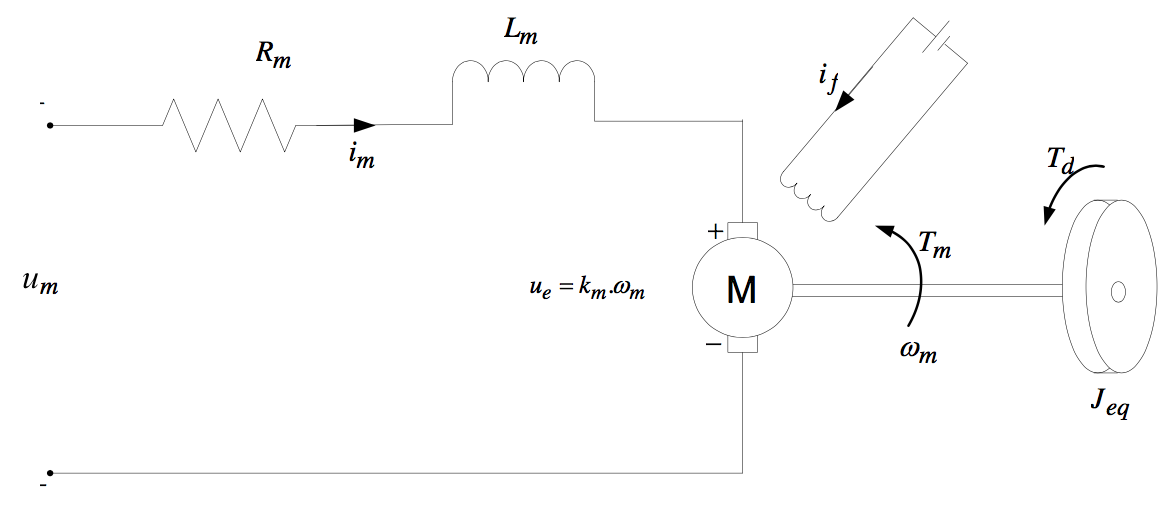
\includegraphics[width=0.7\linewidth]{graphics/motorSchematic}
  \caption{DC Motor in armature configuration}
  \label{fig:motorschematic}
\end{figure}

Table~\ref{table:nomenclature} summarizes the relevant physical parameters in Figure~\ref{fig:motorschematic}.
Relevant equations describing the behavior of the motor will be introduced throughout Section~\ref{sec:results} as they are required.
\begin{table}[htpb]
  \centering
  \caption{DC Motor system nomenclature}
  \label{table:nomenclature}
  \begin{tabular}{@{}clc@{}}
    \toprule
    Symbol & \multicolumn{1}{c}{Description} & Units \\
    \midrule
    $\omega_m$ & Motor angular velocity & \si{\radian\per\second} \\
    $u_m$ & Voltage from amplifier which drives motor & \si{\volt} \\
    $u_e$ & Back-emf voltage & \si{\volt} \\
    $T_d$ & Disturbance torque externally applied to inertial load & \si{\newton\meter} \\
    $T_m$ & Torque generated by motor & \si{\newton\meter} \\
    $i_m$ & Motor armature current & \si{\ampere} \\
    $i_f$ & Motor field current & \si{\ampere} \\
    $k_m$ & Motor torque constant & \si{\newton\meter\per\ampere} \\
    $R_m$ & Motor armature resistance & \si{\ohm} \\
    $L_m$ & Motor armature inductance & \si{\milli\henry} \\
    $J_m$ & Moment of inertia of motor rotor & \si{\kilogram\square\meter} \\
    $J_l$ & Moment of inertia of inertial load & \si{\kilogram\square\meter} \\
    $J_{eq}$ & Total moment of inertia of motor rotor and load & \si{\kilogram\square\meter} \\
    $K$ & Open-loop steady-state gain & \si{\radian\per\volt\per\second} \\
    $\tau$ & Open-loop time constant & \si{\second} \\
    $M_l$ & Inertial load disc mass & \si{\kilogram} \\
    $R_l$ & Inertial load disc radius & \si{\meter} \\
    $s$ & Laplace operator & \si{\radian\per\second} \\
    $t$ & Continuous time & \si{\second} \\
    \bottomrule
  \end{tabular}
\end{table}

